%**************************************************************
% Lab 11: Processor
%**************************************************************
\chapter{Processor}

\section{Purpose}

A \acf{CPU} is arguably one of the most important digital logic devices. \acp{CPU} are found in all computers and many other embedded logic devices. They are versatile circuits that can be used to control many processes and peripheral devices. The purpose of this lab is to lay the foundation of \ac{CPU} operation.

\subsection{A Definition} 

When asked to define ``\ac{CPU}'' many students offer poetic definitions like ``it is the brain of the computer.'' This may be somewhat artistic but is not very helpful in defining \ac{CPU} for digital logic purposes. Here is a much better definition:

\begin{quote}
	A \acf{CPU} is a hardware device that is designed to translate binary codes stored in software into signals that control hardware. Thus, a \ac{CPU} is the interface between software and hardware.
\end{quote}

The purpose of this lab is to demonstrate how binary codes can be used to manipulate hardware devices, like registers and adders, to move data through a circuit and accomplish a purpose. While the circuit developed in this lab is not a practical start for a \ac{CPU} is does serve as an introduction to the concept of hardware manipulation by software codes. 

\section{Procedure}

This processor contains only three subcircuits connected by several bus lines and each of the three subcircuits are reasonably simple to understand.

\subsection{Arithmetic-Logic Unit}

This processor starts with a simple \ac{ALU}, as in Figure \ref{fig:11-01}.

\begin{figure}[H]
	\centering
	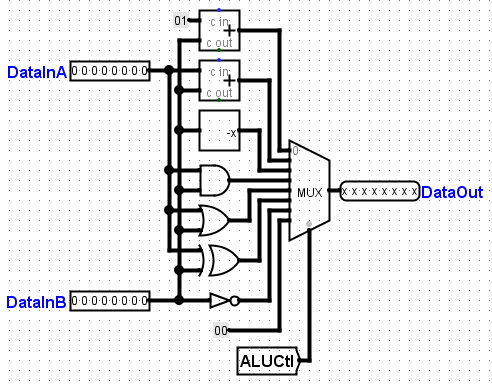
\includegraphics[width=\maxwidth{.95\linewidth}]{gfx/11-01}
	\caption{Simple ALU}
	\label{fig:11-01}
\end{figure}

To be sure, this \ac{ALU} is not very complex but uses the same principles developed in Lab \ref{lab04}, \nameref{lab04}. It contains only three arithmetic functions, increment, add, and negate, four logic functions, \texttt{AND}, \texttt{OR}, \texttt{XOR}, \texttt{NOT}, and one constant zero output. There are two data input ports but note that some of the functions only use the lower input, and one output port. The multiplexer determines which of the functions will be connected to the output and that is controlled by a signal named \textit{ALUCtl}.

The \ac{ALU} is then expanded somewhat to make it usable in a \ac{CPU}.

\begin{figure}[H]
	\centering
	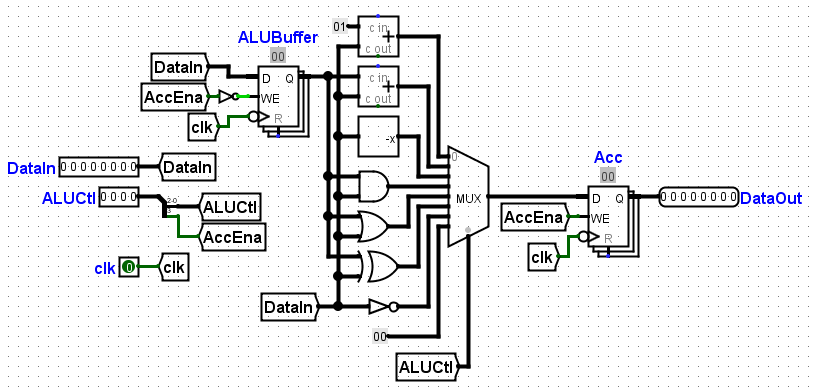
\includegraphics[width=\maxwidth{.95\linewidth}]{gfx/11-02}
	\caption{Full ALU}
	\label{fig:11-02}
\end{figure}

The simple \ac{ALU} functions are found in the center of Figure \ref{fig:11-02}. However, what started as \textit{DataInA} has been replaced by a register named \textit{ALUBuffer}.\footnote{IMPORTANT NOTE: All registers in this Processor circuit are triggered on the Falling Edge of the clock. The reason for this will become evident when the circuit is tested.} The \textit{ALUBuffer's} inputs are from Tunnels (\textit{Wiring} library) because those inputs are used in more than one location in the subcircuit.\footnote{Tunnels are used extensively in this circuit to simplify the diagrams and aid in tracing signals.}

The \ac{ALU} output is routed through a register named \textit{Acc}, for \textit{Accumulator}, which is the commonly-used name for the \ac{ALU} output in a \ac{CPU} circuit.

On the left side of the subcircuit are the three input ports. \textit{DataIn} is an eight-bit number that is sent to both the \textit{ALUBuffer} and the lower \textit{DataIn} bus. The \textit{ALUCtl} signal is split into two components. Bits 0-2 are sent to the multiplexer to select which of the eight functions will be output. Bit 3 of the \textit{ALUCtl} signal is sent to the \textit{AccEna} tunnel and when that is high the \textit{Acc} register will be enabled but when that signal is low then the \textit{ALUBuffer} register will be enabled. Finally, the clock input is sent to both registers.

\subsection{General Registers}

A \ac{CPU} must have several general registers available to hold data while an instruction is being carried out. For example, to temporarily hold the \textit{Acc} output until it is needed in a later step that value can be stored in a register and then recovered when needed. 

The processor circuit being built in this lab has four general registers. Figure \ref{fig:11-03} illustrates the \lstinline[columns=fixed]|GenReg| subcircuit.

\begin{figure}[H]
	\centering
	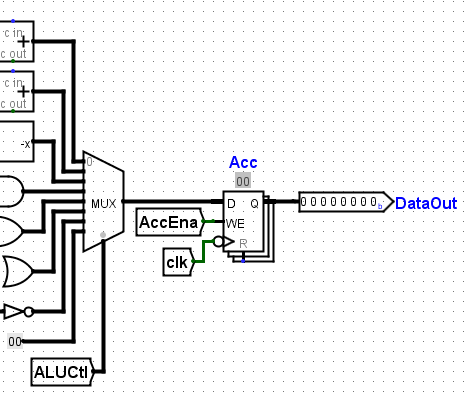
\includegraphics[width=\maxwidth{.95\linewidth}]{gfx/11-03}
	\caption{General Registers}
	\label{fig:11-03}
\end{figure}

The \lstinline[columns=fixed]|GenReg| subcircuit does not require any novel digital logic concepts. Starting on the left side of the circuit:

\begin{itemize}
	\item \textit{DataIn} is connected to the data bus and is the main input port for the registers. Note that \textit{DataIn} is connected to the \textit{Data} port on all four registers. 
	\item The register that actually stores the input data is determined by the Decoder (\textit{Plexers} library) in the lower left corner of the subcircuit. The two low-order bits from the \textit{RegSel} signal activate one of the output lines from the Decoder and that line is tied to the Write Enable port of the register. On the next clock pulse that register will lock in the data present on the \textit{DataIn} port.
	\item The outputs from all of the registers are wired to a Multiplexer (\textit{Plexers} library). The select bits from the Decoder that are used to select the storage register are also used to select the register output line which is, in turn, wired to the \textit{DataOut} port.
	\item The high-order bit from the \textit{RegSel} control signal is used to determine if data are stored to or read from a register. When that bit is high the decoder is active and will select a storage register but when that bit is low the output multiplexer will be activated and send a register's stored value to the output port.
\end{itemize}

\subsection{Control}

The \lstinline[columns=fixed]|Control| subcircuit in this device is very simple and could, in all actuality, be eliminated. However, in a true \ac{CPU} the \lstinline[columns=fixed]|Control| subcircuit is rather complex and critical to the operation of the circuit so a \lstinline[columns=fixed]|Control| subcircuit is included in this lab as an example. Figure \ref{fig:11-04} illustrates the \lstinline[columns=fixed]|Control| subcircuit.

\begin{figure}[H]
	\centering
	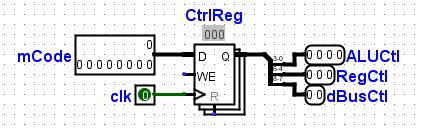
\includegraphics[width=\maxwidth{.95\linewidth}]{gfx/11-04}
	\caption{Control Subcircuit}
	\label{fig:11-04}
\end{figure}

The \lstinline[columns=fixed]|Control| subcircuit includes a nine-bit input named \textit{mCode} (for ``Microcode''). That input is latched by a register\footnote{Note, as an exception to the other registers in the Processor circuit, the register in the control subcircuit must be set to trigger on the leading edge of the clock rather than the falling edge.} and the output of that register is split into three components.

\begin{description}
	\item[Bits 0-3] These are the \ac{ALU} control bits and they are sent to the \lstinline[columns=fixed]|ALU| subcircuit.
	\item[Bits 4-6] These are the register control bits and are sent to that subcircuit.
	\item[Bits 7-8] These are the \textit{dBus} (``Data Bus'') control bits. The data bus is found in the \lstinline[columns=fixed]|main| circuit and carries the data to each of the subcircuits. The dBus control is just a multiplexer that controls which subcircuit's output has control of the data bus.
\end{description}

\subsection{Main}

The \lstinline[columns=fixed]|main| circuit ties the three subcircuits together with three control busses and one data bus. Figure \ref{fig:11-05} illustrates the \lstinline[columns=fixed]|main| circuit.

\begin{figure}[H]
	\centering
	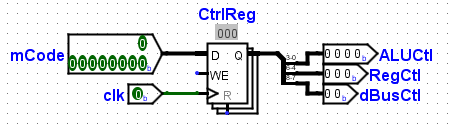
\includegraphics[width=\maxwidth{.95\linewidth}]{gfx/11-05}
	\caption{Main Circuit}
	\label{fig:11-05}
\end{figure}

There are no novel digital logic functions used in this circuit. The first input is \textit{mCode} which is the microcode used to control the flow of data in the dBus (``data bus''). the other input, \textit{LdImm} (``Load Immediate'') can contain an eight-bit number that is to be loaded into one of the registers for processing. In a full \ac{CPU} that input would be wired to a \ac{RAM} device.

\subsection{Testing the Circuit}

The circuit should be tested by inputting these signals and observing the output.

\subsubsection{Copy LdImm To R0}

Enter some value in the \textit{LdImm} input port, set the \textit{mCode} input to 101001000 (the first three values in the table below), and then pulse the \textit{clk}. When completed, the \textit{dBus} and \textit{R0} should both contain the value of the \textit{LdImm} port.

\begin{table}[H]
	\sffamily
	\newcommand{\head}[1]{\textcolor{white}{\textbf{#1}}}		
	\begin{center}
		\rowcolors{2}{gray!10}{white} % Color every other line a light gray
		\begin{tabular}{ccccl} 
			\textbf{dBus} & \textbf{Reg} & \textbf{ALU} & \textbf{dBus} & \textbf{Notes} \\
			10 & 100 & 1000 & LdImm & R0 <- LdImm \\
		\end{tabular}
	\end{center}
	\caption{R0 <- LdImm}
	\label{tab:11-01}
\end{table}

\subsubsection{Copy LdImm To R1}

Enter some value in the \textit{LdImm} input port, set the \textit{mCode} input to 101011000 (the first three values in the table below), and then pulse the \textit{clk}. When completed, the \textit{dBus} and \textit{R1} should both contain the value of the \textit{LdImm} port.

\begin{table}[H]
	\sffamily
	\newcommand{\head}[1]{\textcolor{white}{\textbf{#1}}}		
	\begin{center}
		\rowcolors{2}{gray!10}{white} % Color every other line a light gray
		\begin{tabular}{ccccl} 
			\textbf{dBus} & \textbf{Reg} & \textbf{ALU} & \textbf{dBus} & \textbf{Notes} \\
			10 & 101 & 1000 & LdImm & R1 <- LdImm
		\end{tabular}
	\end{center}
	\caption{R1 <- LdImm}
	\label{tab:11-02}
\end{table}

\subsubsection{Copy LdImm To ALU}

Enter some value in the \textit{LdImm} input port, set the \textit{mCode} input to 100110000 (the first three values in the table below), and then pulse the \textit{clk}. When completed, the \textit{dBus} and \textit{ALU} should both contain the value of the \textit{LdImm} port.

\begin{table}[H]
	\sffamily
	\newcommand{\head}[1]{\textcolor{white}{\textbf{#1}}}		
	\begin{center}
		\rowcolors{2}{gray!10}{white} % Color every other line a light gray
		\begin{tabular}{ccccl} 
			\textbf{dBus} & \textbf{Reg} & \textbf{ALU} & \textbf{dBus} & \textbf{Notes} \\
			10 & 011 & 0000 & LdImm & ALU <- LdImm
		\end{tabular}
	\end{center}
	\caption{ALU <- LdImm}
	\label{tab:11-03}
\end{table}

\subsubsection{Increment dBus}

Set the \textit{mCode} input to 000001000 (the first three values in the table below), and then pulse the \textit{clk}. When completed, the original value of the \textit{dBus} will be incremented by one.

\begin{table}[H]
	\sffamily
	\newcommand{\head}[1]{\textcolor{white}{\textbf{#1}}}		
	\begin{center}
		\rowcolors{2}{gray!10}{white} % Color every other line a light gray
		\begin{tabular}{ccccl} 
			\textbf{dBus} & \textbf{Reg} & \textbf{ALU} & \textbf{dBus} & \textbf{Notes} \\
			00 & 000 & 1000 & dBus+1 & dBus <- Inc(dBus)
		\end{tabular}
	\end{center}
	\caption{dBus <- Inc(dBus)}
	\label{tab:11-04}
\end{table}

\subsubsection{Add R0 And R1, Store In R0}

\marginpar{Use the LdImm function to initialize R0 and R1.}Adding the values of \textit{R0} and \textit{R1} and storing the result in \textit{R0} requires three steps. Set the \textit{mCode} input to the first three values in the table below and pulse the \textit{clk} for each of the steps. When completed, the sum of the original values of \textit{R0} and \textit{R1} will be stored in \textit{R0}.

\begin{table}[H]
	\sffamily
	\newcommand{\head}[1]{\textcolor{white}{\textbf{#1}}}		
	\begin{center}
		\rowcolors{2}{gray!10}{white} % Color every other line a light gray
		\begin{tabular}{ccccl} 
			\textbf{dBus} & \textbf{Reg} & \textbf{ALU} & \textbf{dBus} & \textbf{Notes} \\
			01 & 001 & 0001 & R1 & ALU <- R1 \\
			01 & 000 & 1001 & R0 & Acc <- R0 + R1 \\
			00 & 100 & 0001 & Acc & R0 <- Acc 
		\end{tabular}
	\end{center}
	\caption{R0 <- R0 + R1}
	\label{tab:11-05}
\end{table}

\subsubsection{Subtract R1 From R0, Store In R0}

\marginpar{Use the LdImm function to initialize R0 and R1.}Subtracting the value of \textit{R1} from \textit{R0} and storing the result in \textit{R0} requires four steps. Set the \textit{mCode} input to the first three values in the table below and pulse the \textit{clk} for each of the steps. When completed, the difference of the original values of \textit{R0} and \textit{R1} will be stored in \textit{R0}.

\begin{table}[H]
	\sffamily
	\newcommand{\head}[1]{\textcolor{white}{\textbf{#1}}}		
	\begin{center}
		\rowcolors{2}{gray!10}{white} % Color every other line a light gray
		\begin{tabular}{ccccl} 
			\textbf{dBus} & \textbf{Reg} & \textbf{ALU} & \textbf{dBus} & \textbf{Notes} \\
			01 & 000 & 0010 & R0 & ALU <- R0 \\
			01 & 001 & 1010 & R1 & Acc <- \textasciitilde R1 \\
			00 & 100 & 1001 & R0-R1 & dBus <- Acc \\
			00 & 100 & 0111 & dBus+1 & R0 <- R0 - R1
		\end{tabular}
	\end{center}
	\caption{R0 <- R0 - R1}
	\label{tab:11-06}
\end{table}

\subsubsection{Copy R0 to R1}

\marginpar{Use the LdImm function to initialize R0.}Copying the value of \textit{R0} to \textit{R1} requires four steps. Set the \textit{mCode} input to the first three values in the table below and pulse the \textit{clk} for each of the steps. When completed, the value of \textit{R0} will be stored in \textit{R1}.

\begin{table}[H]
	\sffamily
	\newcommand{\head}[1]{\textcolor{white}{\textbf{#1}}}		
	\begin{center}
		\rowcolors{2}{gray!10}{white} % Color every other line a light gray
		\begin{tabular}{ccccl} 
			\textbf{dBus} & \textbf{Reg} & \textbf{ALU} & \textbf{dBus} & \textbf{Notes} \\
			00 & 000 & 1111 & 0 & dBus <- 0 \\
			00 & 000 & 0100 & 0 & ALU <- dBus \\
			01 & 000 & 1100 & Acc & Acc <- ALU OR R0 \\
			00 & 101 & 0111 & Acc & R1 <- Acc
		\end{tabular}
	\end{center}
	\caption{R1 <- R0}
	\label{tab:11-07}
\end{table}

\subsubsection{Swap R0 And R1}

\marginpar{Use the LdImm function to initialize R0 and R1.}Swapping the values of \textit{R0} and \textit{R1} requires 12 steps. Set the \textit{mCode} input to the first three values in the table below and pulse the \textit{clk} for each of the steps. When completed, the values of \textit{R0} and \textit{R1} will exchanged.

\begin{table}[H]
	\sffamily
	\newcommand{\head}[1]{\textcolor{white}{\textbf{#1}}}		
	\begin{center}
		\rowcolors{2}{gray!10}{white} % Color every other line a light gray
		\begin{tabular}{ccccl} 
			\textbf{dBus} & \textbf{Reg} & \textbf{ALU} & \textbf{dBus} & \textbf{Notes} \\
			00 & 000 & 1111 & 0 & dBus <- 0 (Move R0 to R2)\\
			00 & 000 & 0100 & 0 & ALU <- dBus \\
			01 & 000 & 1100 & Acc & Acc <- ALU OR R0 \\
			00 & 110 & 0111 & Acc & R2 <- Acc \\
 			& & & & \\ %Empty line

			00 & 000 & 1111 & 0 & dBus <- 0 (Move R1 to R0)\\
			00 & 000 & 0100 & 0 & ALU <- dBus \\
			01 & 001 & 1100 & Acc & Acc <- ALU OR R1 \\
			00 & 100 & 0111 & Acc & R0 <- Acc \\
 			& & & & \\ %Empty line

			00 & 000 & 1111 & 0 & dBus <- 0 (Move R2 to R1)\\
			00 & 000 & 0100 & 0 & ALU <- dBus \\
			01 & 010 & 1100 & Acc & Acc <- ALU OR R2 \\
			00 & 101 & 0111 & Acc & R1 <- Acc
		\end{tabular}
	\end{center}
	\caption{R0 <-> R1}
	\label{tab:11-08}
\end{table}

\section{About Programming Languages}

The codes that were input for the last example (swap \textit{R0} and \textit{R1}) would create the following program.

\begin{Verbatim}[frame=lines,
xleftmargin=10mm,
xrightmargin=10mm]
000001111
000000100
010001100
001100111
000001111
000000100
010011100
001000111
000001111
000000100
010101100
001010111
\end{Verbatim}

This group of instructions would be considered ``CPU Microcode,'' which is a very highly specialized form of programming. It is the code that is built into a \ac{CPU} circuit and it determines what gates, registers, and other devices are active for each step of the code. When Intel, AMD, Motorola, or other manufacturers create a new \ac{CPU}, one of their main challenges is creating the microcode that will, for example, ``add the contents of register one to the contents of register two and store the result in register zero.'' The microcode must be able to activate and deactivate various devices within the \ac{CPU} so data appear on the appropriate bus at the right time in order to achieve the objective. Normally, microcode steps must be executed over several clock cycles in order to do a single job. For example, in one clock cycle the contents of register one may be placed on the data bus, the next clock cycle will load that data into the ALU register, and so forth until the entire process is complete.

Microcode is usually stored in \ac{ROM} that is built into the \ac{CPU}. This is typically called ``firmware'' since it is a string of ones and zeros, like software, but it cannot be changed, like hardware.

It is important to keep in mind the difference between instructions contained in a software program (like Word) and those contained in microcode. A single instruction in software is interpreted and executed by the \ac{CPU} using, perhaps, dozens of microcode steps. As an example, the software may want to move a single byte from \ac{RAM} to the video card. The \ac{CPU} may process that instruction by first moving the byte from \ac{RAM} to register one and then moving it from there to the video card's input register. Those moves may require several clock cycles as various multiplexers and other devices are activated in the correct sequence to move the data to its destination. 

In summary, the CPU's Control Unit controls all of the registers, buffers, buses, and other devices in the CPU in order to execute the instructions requested by the software program.

A computer program, as contained in software, is nothing more than a series of ones and zeros, organized into groups of 32 (or 64). Each group of bits forms a single ``word'' of information; or a single instruction which would then be used to trigger a microcode sequence within the \ac{CPU}. When viewed at the level of ones and zeros, a program is said to be in ``machine code,'' and could look something like this:

\begin{Verbatim}[frame=lines,
xleftmargin=10mm,
xrightmargin=10mm]
10010100101100101001101011001010
01101001101011000111101011101011
00011011110010000111010111100101
\end{Verbatim}

If a programmer could master machine code, then those programs would be as concise and efficient as possible since they would be written in machine code the \ac{CPU} can execute directly. Of course, as it is easy to imagine, no one actually writes machine code due to its complexity.

The next level higher than machine code is called ``Assembly'' code. Assembly uses easy-to-remember abbreviations to represent the various \ac{CPU} instructions available; and it looks something like this: 

\begin{Verbatim}[frame=lines,
xleftmargin=10mm,
xrightmargin=10mm]
INP
STA FIRST 
INP
STA SECOND 
LDA FIRST 
SUB SECOND
OUT
HLT
FIRST DAT
SECOND DAT
\end{Verbatim}

Once the program has been written in Assembly, it must be ``assembled'' into machine code before it can be executed. An assembler is a fairly simply program that converts a file containing assembly codes into machine codes that can be executed by the \ac{CPU}.

Many programming languages have been developed that are considered ``higher'' than Assembly; for example, C++, Java, and Visual Basic. These languages tend to be easy to master and can enable a programmer to quickly create very complex programs. Programs written in each of these languages must be compiled, or changed into machine code, before they can be executed. Here is an example Java program:

\begin{Verbatim}[frame=lines,
xleftmargin=10mm,
xrightmargin=10mm]
public class HelloWorldExample{
  public static void main(String args[]){
  System.out.println("Hello World !"); 
  }
}
\end{Verbatim}

In the end, while there are dozens of different programming languages, they are all designed to be reduced into a series of machine codes, which the \ac{CPU} can then execute.

\section{Challenge}

Using the examples in the ``Testing the Circuit'' section, create the microcode necessary to carry out these functions:

\begin{enumerate}
	\item Store the value contained in \textit{LdImm} in \textit{R2} (\textit{R2} <- \textit{LdImm}). (Assume that \textit{LdImm} is pre-loaded with the value to store.)
	\item Store the value contained in \textit{LdImm} in \textit{R3} (\textit{R3} <- \textit{LdImm}). (Assume that \textit{LdImm} is pre-loaded with the value to store.)
	\item Store the 2s complement of the value in \textit{R0} back into \textit{R0} (\textit{R0} <- \textasciitilde \textit{R0}). The subtraction example will help with this function.
	\item Store the bitwise NOT of the value in \textit{R0} back into \textit{R0} (\textit{R0} <- \textit{R0'}).
\end{enumerate}

\section{Deliverable}

To receive a grade for this lab, build the Processor circuit and then complete the Challenge. Be sure the standard identifying information is at the top left of the Processor \lstinline{main} circuit, similar to: 

\bigskip
% The minipage environment keeps the three lines together - no page break.
\begin{minipage}{\linewidth}
	\begin{verbatim}
	George Self
	Lab 11: Processor
	April 5, 2018
	\end{verbatim}
\end{minipage}
\bigskip

Save the Processor circuit in a file with this name: \textit{Lab11\_Processor}. Complete the code required in the Challenge and store that in a text file with the name \textit{Lab11\_Code.txt}. Submit both files for grading.
